\chapter{Map}\label{ch:map}

% Definition.
The \termdef{map}[Map] is the static geometry of the \termref{battlefield}[Battlefield], comprised of a \termref{grid}[Map!Grid] of \termref{tiles}[Map!Tile].

% Requirements.
For simplicity, we allow maps to contain holes, but require all other \termref{tiles}[Map!Tile] on it to be \termref{connected}[Map!Connection].

\section{Grid}

% Definition.
The \termdef{map grid}[Map!Grid] is a two-dimensional space-filling tiling that establishes a discrete integer coordinate system.

\subsection{Tile}

% Definition.
A \termdef{map tile}[Map!Tile] is the smallest distinguishable element of the \termref{grid tiling}[Map!Grid].
We define our tiles to be hexagons as depicted in~\ref{fig:map_tile}.

% Draw a hexagon.
%   \hexcell{q}{r}[text=][walls=0]
\NewDocumentCommand{\hexcell}{mmO{}O{0}}{%
\begin{scope}[shift={(1.5*#1,0.86602540378*(-#1-2*#2))}]%chktex 36, chktex 8
\draw (0:1) \foreach \x in {60,120,...,360} {-- (\x:1)};%chktex 1, chktex 11
\node (q#1r#2) at (0,0) {#3};%chktex 1
\draw[line width={1mm*Mod(#4,2)}] (120:1) -- (60:1);%chktex 36, chktex 8
\draw[line width={1mm*Mod(div(#4,2),2)}] (60:1) -- (0:1);%chktex 36, chktex 8
\draw[line width={1mm*Mod(div(#4,4),2)}] (0:1) -- (-60:1);%chktex 36, chktex 8
\end{scope}%
}
% Draw a filled hexagon.
%   \hexfill{q}{r}[color=black]
\NewDocumentCommand{\hexfill}{mmO{black}}{%
\begin{scope}[shift={(1.5*#1,0.86602540378*(-#1-2*#2))}]%chktex 36, chktex 8
\fill[#3] (0:0.9) \foreach \x in {60,120,...,360} {-- (\x:0.9)};%chktex 1, chktex 11
\end{scope}%
}

% Figure: Tile.
\begin{figure}[htbp]
    \centering
    \begin{tikzpicture}
        \hexcell{0}{0}
    \end{tikzpicture}
    \caption{Tile}\label{fig:map_tile}
\end{figure}

\subsection{Coordinates}

% (q, r) coordinates.
Let \(Q\) and \(R\) be two distinct symmetry axes out of the three of the \termref{tile}[Map!Tile] (see~\ref{fig:map_tile_axes}).
We define the \termdef{coordinate space}[Map!Coordinates] \(\mathbf{C}\) to be the set of all axis coordinate pairs \((q, r)\):

\begin{equation}\label{eq:map_coords_qr}
    \mathbf{C} := \left \{ (q, r) \in \mathbb{Z}^2 \right \}
\end{equation}

% Figure: Symmetry axes.
\begin{figure}[htbp]
    \centering
    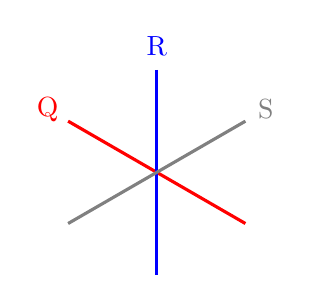
\begin{tikzpicture}
        \hexcell{0}{0}

        % Q.
        \draw[red, line width=0.4mm] (150:1.3) -- (-30:1.3);
        \node[red] at (150:1.6) {Q};
        % R.
        \draw[blue, line width=0.4mm] (90:1.3) -- (-90:1.3);
        \node[blue] at (90:1.6) {R};
        % S.
        \draw[gray, line width=0.4mm] (30:1.3) -- (-150:1.3);
        \node[gray] at (30:1.6) {S};
    \end{tikzpicture}
    \caption{Tile axes}\label{fig:map_tile_axes}
\end{figure}

% (q, r, s) coordinates.
Let the remaining symmetry axis be called \(S\) with an associated coordinate \(s\), and we observe that our defined coordinate system satisfies:

\begin{equation}\label{eq:map_coords_sum}
    q + r + s = 0
\end{equation}

% s coordinate derivation.
Consequently, we can transform~\eqref{eq:map_coords_sum} to derive the correct \(s\) coordinate for any pair of coordinates \((q, r)\):

\begin{equation}\label{eq:map_coords_s}
    a_s := -a_q - a_r\text{ for \(a \in \mathbf{C}\)}
\end{equation}

% Coordinate operations.
We can now define (without proof) the coordinate operations over \(\mathbf{C}\), such that we define a coordiante vector space as depicted in~\ref{fig:map_coords}:

\begin{align*}
    -a &= (-a_q, -a_r)&\\
    a + b &= (a_q + b_q, a_r + b_r)&\\
    a - b &= a + -b&\\
    k a &= (k a_q, k a_r)&\\
    &&\text{with \(a, b \in \mathbf{C}, k \in \mathbf{Z}\)}
\end{align*}

% Figure: Map coordinates.
\begin{figure}[htbp]
    \centering
    \begin{tikzpicture}
        % Q label
        \node[red] (Q) at (90:4) {$Q=0$};
        \draw[red, line width=0.4mm,shift=(Q)] (-90:0.4) -- (-90:1.3);
        \draw[red,dotted,line width=0.2mm,shift=(Q)] (-90:1.4) -- (-90:8.3);
        % R label
        \node[blue] (R) at (150:4) {$R=0$};
        \draw[blue, line width=0.4mm,shift=(R)] (-30:0.4) -- (-30:1.3);
        \draw[blue,dotted,line width=0.2mm,shift=(R)] (-30:1.4) -- (-30:10);

        % Col -1
        \hexcell{-1}{0}[-1, 0]
        \hexcell{-1}{1}[-1, 1]
        \hexcell{-1}{2}[-1, 2]

        % Col 0
        \hexcell{0}{-1}[0, -1]
        \hexcell{0}{0}[0, 0]
        \hexcell{0}{1}[0, 1]
        \hexcell{0}{2}[0, 2]

        % Col 1
        \hexcell{1}{-1}[1, -1]
        \hexcell{1}{0}[1, 0]
        \hexcell{1}{1}[1, 1]

        % Col 2
        \hexcell{2}{-2}[2, -2]
        \hexcell{2}{-1}[2, -1]
        \hexcell{2}{0}[2, 0]
        \hexcell{2}{1}[2, 1]

        % Col 3
        \hexcell{3}{-2}[3, -2]
        \hexcell{3}{-1}[3, -1]
        \hexcell{3}{0}[3, 0]
    \end{tikzpicture}
    \caption{Map coordinates}\label{fig:map_coords}
\end{figure}

\subsection{Distance}

% L1.
Given two coordinates \(a\) and \(b\), the \(L_1\) distance in our \termref{grid}[Map!Grid] now reads:

\begin{equation}\label{eq:map_dist_qrs}
    |a - b| = \max\left \{
        |\underbrace{a_q - b_q}_{dq}|,
        |\underbrace{a_r - b_r}_{dr}|,
        |\underbrace{a_s - b_s}_{ds}|
    \right \}
\end{equation}

% Remove ds.
Substituting with~\eqref{eq:map_coords_s}, we can derive \(ds\) from \(dq\) and \(dr\) as follows:

\begin{align}\label{eq:map_dist_ds}
    d_s &= (-a_q - a_r) - (-b_q - b_r)\nonumber \\
    &= b_q - a_q + b_r - a_r\nonumber \\
    &= -dq - dr
\end{align}

% Definition.
Applying this result to~\eqref{eq:map_dist_qrs}, we define the \termdef{distance}[Map!Distance] between two \termref{tiles}[Map!Tile] as the \(L_1\) distance:

\begin{align}\label{eq:map_dist_qr}
    |a - b| &= \max\left \{ |dq|, |dr|, |-dq-dr| \right \}\nonumber \\
    |a - b| &= \max\left \{ |dq|, |dr|, |dq+dr| \right \} \\
\end{align}

% Unit.
Distance is measured in units (\mapunit{}). The distance between two \termref{adjacent tiles}[Map!Adjacency] is \SI{1}{\mapunits}.

\subsection{Adjacency}

% Definition.
We define the \termdef{adjacency relation}[Map!Adjacency] over pairs of \termref{tiles}[Map!Tile] identified by their \termref{coordinates}[Map!Coordinates] as follows:

\begin{align}\label{eq:map_adj}
    a \overset{adj}{\leftrightarrow} b &\iff |a - b| = 1\\
    &\iff (a_q - b_q = 0)
        \vee (a_r - b_r = 0)
        \vee (a_q - b_q = -a_q + b_q)\nonumber
\end{align}

% Properties.
Therefore, the following properties are also guaranteed:

\begin{align*}
    a \overset{adj}{\leftrightarrow} b &\implies
        b \overset{adj}{\leftrightarrow} a&\textit{(symmetric)}\\
    a \overset{adj}{\leftrightarrow} b &\implies
        a \neq b&\textit{(not reflexive)}
\end{align*}

\subsection{Direction}

% Definition.
Given a pair of \termref{adjacent tiles}[Map!Adjacency] \((a, b)\), we define the \termdef{cardinal direction}[Map!Direction] of \(b\) relative to \(a\) according to~\ref{fig:map_dirs}.

% Figure: Map directions.
\begin{figure}[htbp]
    \centering
    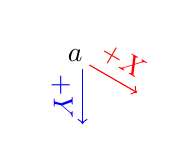
\begin{tikzpicture}
        % Fixed a.
        \hexcell{0}{0}[\(a\)]

        % X axis indicator.
        \draw[->,red] (-30:0.1) -- (-30:0.8) node[midway,sloped,above] {\(+X\)};
        % Y axis indicator.
        \draw[->,blue] (-90:0.1) -- (-90:0.8) node[midway,sloped,below] {\(+Y\)};

        % All bs.
        \hexcell{0}{-1}[N]
        \hexcell{1}{-1}[NE]
        \hexcell{1}{0}[SE]
        \hexcell{0}{1}[S]
        \hexcell{-1}{1}[SW]
        \hexcell{-1}{0}[NW]
    \end{tikzpicture}
    \caption{Map directions}\label{fig:map_dirs}
\end{figure}

\section{Walls}

% Definition.
A \termdef{wall}[Map!Wall] is a specially designated edge shared between two \termref{tiles}[Map!Tile].
Every edge in the \termref{grid}[Map!Grid] can be a wall.

% Simplification.
In order to simplify the definition of walls, and to avoid redundancies, we define that every \termref{tiles}[Map!Tile] declares a set of associated walls, which may contain the \termref{N}[Map!Direction], \termref{NE}[Map!Direction] and \termref{SE}[Map!Direction] edges, as depcited in~\ref{fig:map_walls}, in any combination.

% Figure: Map walls.
\begin{figure}[htbp]
    \centering
    \begin{subfigure}{0.3\textwidth}
        \centering
        \begin{tikzpicture}
            \hexcell{0}{0}[][1]
        \end{tikzpicture}
        \caption{N wall}
    \end{subfigure}
    \begin{subfigure}{0.3\textwidth}
        \centering
        \begin{tikzpicture}
            \hexcell{0}{0}[][2]
        \end{tikzpicture}
        \caption{NE wall}
    \end{subfigure}
    \begin{subfigure}{0.3\textwidth}
        \centering
        \begin{tikzpicture}
            \hexcell{0}{0}[][4]
        \end{tikzpicture}
        \caption{SE wall}
    \end{subfigure}
    \caption{Map walls}\label{fig:map_walls}
\end{figure}

% Completeness.
Given these rules, it is easily proven that all other possible edges can also be walled.
Following the observation that walls are always shared by two \termref{adjacent tiles}[Map!Adjacency], we notice that they can be substituted for any \termref{tile}[Map!Tile] as follows:

\begin{itemize}
    \item [S] {\(\rightarrow \) N wall of S \termref{adjacent tile}[Map!Adjacency]}
    \item [SW] {\(\rightarrow \) NE wall of SW \termref{adjacent tile}[Map!Adjacency]}
    \item [NW] {\(\rightarrow \) SE wall of NW \termref{adjacent tile}[Map!Adjacency]}
\end{itemize}

\subsection{Link}

% Definition.
Given a pair of \termref{adjacent tiles}[Map!Adjacency] \((a,b)\), they are \termdef{linked}[Map!Link] if and only if their shared edge is not a \termref{wall}[Map!Wall] as shown in~\ref{fig:map_link}.

% Notation.
We denote this relation as \(a \overset{lnk}{\leftrightarrow} b\), with the following observed properties:

\begin{align*}
    a \overset{lnk}{\leftrightarrow} b &\implies
        b \overset{lnk}{\leftrightarrow} a&\textit{(symmetric)}\\
    a \overset{lnk}{\leftrightarrow} b &\implies
        a \neq b&\textit{(not reflexive)}
\end{align*}

% Figure: Tile link.
\begin{figure}[htbp]
    \centering
    \begin{subfigure}{0.48\textwidth}
        \centering
        \begin{tikzpicture}
            \hexcell{0}{0}
            \hexcell{1}{-1}

            % Unblocked path.
            \draw[<->,line width=0.4mm] (q0r0) -- (q1r-1);
        \end{tikzpicture}
        \caption{linked tiles}
    \end{subfigure}
    \begin{subfigure}{0.48\textwidth}
        \centering
        \begin{tikzpicture}
            \hexcell{0}{0}[][2]
            \hexcell{1}{-1}

            % NE blocked path.
            \draw[-{Bar},line width=0.4mm] (0, 0) -- (30:0.7);
            % SW blocked path.
            \begin{scope}[shift={(q1r-1)}]
                \draw[-{Bar},line width=0.4mm] (0, 0) -- (-150:0.7);
            \end{scope}
        \end{tikzpicture}
        \caption{blocked link}
    \end{subfigure}
    \caption{Tile links}\label{fig:map_link}
\end{figure}

\section{Primitives}

% Explanation.
Frome the above definitions, we derive a set of primitive shapes, which are parameterized sets of tiles, for use in more advanced definitions.
Each primitive pertains to one or more parent tiles that span it.

\subsection{Path}

% Definition.
A \termdef{path}[Map!Path] \(P\) is a sequence of \termref{tiles}[Map!Tile] identified by their \termref{coordinates}[Map!Coordinates] \((p_1, p_2, \ldots, p_N)\) with length \(|P| = N\) such that:

\begin{align}\label{eq:map_path}
    \forall i \in \interval[open right]{1}{N} &:
        p_i \overset{lnk}{\leftrightarrow} p_{i+1}&\textit{(linked)}
\end{align}

% Reversability.
It is trivially shown that reversing a path, that is inverting the order of its \termref{tiles}[Map!Tile], always yields a valid path:

\begin{align}\label{eq:map_path_rev}
    (p_N, p_{N-1}, \ldots, p_1)\text{ is a path} &\impliedby
        \forall i \in \interval{2}{N} :
            p_i \overset{lnk}{\leftrightarrow} p_{i-1}\nonumber \\
    &\impliedby
        \forall i \in \interval{2}{N} :
            p_{i-1} \overset{lnk}{\leftrightarrow} p_i\nonumber \\
    &\impliedby
        \forall i \in \interval[open right]{1}{N} :
            p_i \overset{lnk}{\leftrightarrow} p_{i+1}\nonumber \\
    &\impliedby (p_1, p_2, \ldots, p_N)\text{ is a path}
\end{align}

% Equality.
Let \(P\) and \(Q\) be two paths of length \(N\).
We define the equality relation for these paths as follows:

\begin{equation}\label{eq:map_path_eq}
    P = Q \iff \forall i \in \interval[open right]{1}{N} : p_i = q_i
\end{equation}

% Parameterization.
Additionally, we define a parameterized path \(P_{a,b}\) to be a path \((a, p_2, \ldots, p_{N-1}, b)\), referred to as the path \emph{from} \(a\) \emph{to} \(b\).

% Ambiguity.
For any pair of tiles \((a,b)\) there might be multiple such paths \(P_{a,b}\) that differ in length, such as shown in~\ref{fig:map_path}.

% Figure: Map path.
\begin{figure}[htbp]
    \centering
    \begin{tikzpicture}
        \hexcell{0}{0}[a]
        \hexcell{1}{-1}
        \hexcell{1}{0}[][2]
        \hexcell{2}{-2}
        \hexcell{2}{-1}[][2]
        \hexcell{2}{0}[][7]
        \hexcell{3}{-2}
        \hexcell{3}{-1}[][7]
        \hexcell{3}{0}[][2]
        \hexcell{4}{-2}[b]
        \hexcell{4}{-1}[][6]
        \hexcell{4}{0}[][1]
        \hexcell{5}{-2}
        \hexcell{5}{-1}

        % Shortest path.
        \path[shift=(q0r0)] (30:0.2) coordinate (start);
        \path[shift=(q4r-2)] (150:0.2) coordinate (end);
        \draw[->, red, line width=0.4mm] plot [smooth] coordinates {(start) (q1r-1) (q2r-2) (q3r-2) (end)};
        \node[red] at (0,1.3) {$N=5$};
        % Alternative path.
        \path[shift=(q4r-2)] (-30:0.2) coordinate (end);
        \draw[->, blue, line width=0.4mm] plot [smooth] coordinates {(start) (q1r-1) (q2r-1) (q3r-1) (q3r0) (q4r0) (q5r-1) (q5r-2) (end)};
        \node[blue] at (0,-1.3) {$N=9$};
    \end{tikzpicture}
    \caption{Map path}\label{fig:map_path}
\end{figure}

% Shortest paths.
We define the set of \emph{shortest paths} \(P'_{a,b}\) between \(a\) and \(b\) to be:

\begin{align}\label{eq:map_path_short}
    \|P'_{a,b}\| &:= \min\left \{ +\infty, |P_{a,b}| \right \}\nonumber \\
    P'_{a,b} &:= \left \{ x \in \left \{ P_{a,b} \right \} :
        |x| = \|P'_{a,b}\|
    \right \}
\end{align}

Where \( \|P'_{a,b}\| \) denotes the \emph{shortest path length}, which defaults to \(+\infty \) if there is no path between \(a\) and \(b\).

% Connectivity
Finally, we introduce the \termdef{connection}[Map!Connection] relation between two \termref{tiles}[Map!Tile] \(a\) and \(b\) if and only if there exists a path between them:

\begin{equation}
    a \overset{con}{\leftrightarrow} b \iff \exists P_{a,b}\\
\end{equation}

% Properties.
We observe the following properties of this relation:

\begin{align*}
    a \overset{con}{\leftrightarrow} b &\implies
        b \overset{con}{\leftrightarrow} a&\textit{(symmetric)}\\
    a \overset{con}{\leftrightarrow} b &\implies
        a \neq b&\textit{(not reflexive)}
\end{align*}

\subsection{Neighborhood}

% Definition.
The \termdef{neighborhood}[Map!Neighborhood] \(N_{C,r}\) with radius \(r\) around a \termref{tile}[Map!Tile] identified by its \termref{coordinates}[Map!Coordinates] \(C\) is a set of \termref{coordinates}[Map!Coordinates] \(n\) such that:

\begin{equation}\label{eq:map_nbhd}
    N := \left \{ n \in \mathbf{C} : |n - C| \leq r \right \}
\end{equation}

% Properties.
It is trivially shown that \(C \in N_{C,r}\) for any \(r \geq 0\).
See~\ref{fig:map_nbhd} for a graphical representation of a neighborhood.

% Size.
The size of \(N_{C,r}\) with \(r \geq 0\) solely depends on \(r\), given by the formula:

\begin{align}\label{eq:map_nbhd_size}
    |N_{C,r}| &= 1 + 6\sum_{i=1}^{r}i\nonumber \\
    &= 1 + \frac{6r(1 + r)}{2}\nonumber \\
    &= 3r^2 + 3r + 1
\end{align}

% Figure: Tile neighborhood.
\begin{figure}[htbp]
    \centering
    \begin{tikzpicture}
        % d<=0
        \hexcell{0}{0}[C]
        \draw[line width=0.4mm] (0,0) circle (0.4);
        \node at (90:0.65) {$d\leq0$};

        % d<=1
        \hexcell{0}{-1}
        \hexcell{1}{-1}
        \hexcell{1}{0}
        \hexcell{0}{1}
        \hexcell{-1}{1}
        \hexcell{-1}{0}
        \draw[red, line width=0.4mm] plot [smooth cycle] coordinates {(q0r-1) (q1r-1) (q1r0) (q0r1) (q-1r1) (q-1r0)};
        \node[red] at (90:2) {$d\leq1$};

        % d<=2
        \hexcell{0}{-2}
        \hexcell{1}{-2}
        \hexcell{2}{-2}
        \hexcell{2}{-1}
        \hexcell{2}{0}
        \hexcell{1}{1}
        \hexcell{0}{2}
        \hexcell{-1}{2}
        \hexcell{-2}{2}
        \hexcell{-2}{1}
        \hexcell{-2}{0}
        \hexcell{-1}{-1}
        \draw[blue, line width=0.4mm] plot [smooth cycle] coordinates {(q0r-2) (q1r-2) (q2r-2) (q2r-1) (q2r0) (q1r1) (q0r2) (q-1r2) (q-2r2) (q-2r1) (q-2r0) (q-1r-1)};
        \node[blue] at (90:3.8) {$d\leq2$};
    \end{tikzpicture}
    \caption{Tile neighborhood \(N_{C=(0,0),r=2}\)}\label{fig:map_nbhd}
\end{figure}

\subsection{Perimeter}

% Definition.
The \termdef{perimeter}[Map!Perimeter] \(O_{C,r}\) with radius \(r\) around a \termref{tile}[Map!Tile] identified by its \termref{coordinates}[Map!Coordinates] \(C\) is a set of \termref{coordinates}[Map!Coordinates] \(o\) such that:

\begin{equation}\label{eq:map_peri}
    O := \left \{ o \in \mathbf{C} : |o - C| = r \right \}
\end{equation}

% Properties.
It is trivially shown that \(C \notin V_{C,r}\) for any \(r > 0\).
See~\ref{fig:map_peri} for a graphical representation of a perimeter.

% Size.
The size of \(O_{C,r}\) with \(r \geq 0\) solely depends on \(r\), given by the formula:

\begin{equation}\label{eq:map_peri_size}
    |O_{C,r}| = \begin{cases}
        6r & r > 0\\
        1 & r = 0
    \end{cases}
\end{equation}

% Figure: Tile perimeter.
\begin{figure}[htbp]
    \centering
    \begin{tikzpicture}
        % C
        \node at (0,0) {C};

        % d<=2
        \hexcell{0}{-2}
        \hexcell{1}{-2}
        \hexcell{2}{-2}
        \hexcell{2}{-1}
        \hexcell{2}{0}
        \hexcell{1}{1}
        \hexcell{0}{2}
        \hexcell{-1}{2}
        \hexcell{-2}{2}
        \hexcell{-2}{1}
        \hexcell{-2}{0}
        \hexcell{-1}{-1}
        \draw[blue, line width=0.4mm] plot [smooth cycle] coordinates {(q0r-2) (q1r-2) (q2r-2) (q2r-1) (q2r0) (q1r1) (q0r2) (q-1r2) (q-2r2) (q-2r1) (q-2r0) (q-1r-1)};
        \node[blue] at (90:3.8) {$d=2$};
    \end{tikzpicture}
    \caption{Tile perimeter \(P_{C=(0,0),r=2}\)}\label{fig:map_peri}
\end{figure}

\subsection{Ray}

% Definition.
A \termdef{ray}[Map!Ray] \(R_{A,B}\) between two \termref{tiles}[Map!Tile] identified by their \termref{coordinates}[Map!Coordinates] \(A\) and \(B\) is a set \termref{coordinates}[Map!Coordinates] \(r\) such that:

\begin{equation}\label{eq:map_ray}
    R_{A,B} := \left \{ r \in \mathbf{C} :
        r_q = \lfloor A_q + t(B_q-A_q) \pm w \rfloor,
        r_r = \lfloor A_r + t(B_r-A_r) \pm w \rfloor
    \right \}
\end{equation}
\begin{align*}
    t &= \frac{i}{|A-B|}\text{ with \(i \in \interval{0}{|A-B|} \subset \mathbb{Z}\)}\\
    w &\approx 0.1
\end{align*}

% Raytracing.
Where \(t\) is the fractional ray distance, evaluated in samples \(|A-B|\) with indices \(i\).

% Ray width.
Rays are used in raycasting, which determines the \termref{coordinates}[Map!Coordinates] of all \termref{tiles}[Map!Tile] along a ray on the \termref{map}[Map].
To resolve ambiguities when sampling on \termref{tiles}[Map!Tile] edges, we introduce the ray width \(0 < w \ll 1\), which results in rays as depcited in~\ref{fig:map_ray}.

% Figure: Ray width.
\begin{figure}[htbp]
    \centering
    \begin{subfigure}{0.48\textwidth}
        \centering
        \begin{tikzpicture}
            \hexcell{0}{0}[A]
            \hexcell{0}{-1}
            \hexcell{1}{-1}
            \hexcell{1}{-2}[B]

            \path[shift=(q0r0)] (60:0.3) coordinate (start);
            \path[shift=(q1r-2)] (-120:0.3) coordinate (end);
            \draw[<->, line width=2mm] (start) -- (end);
        \end{tikzpicture}
    \end{subfigure}
    \begin{subfigure}{0.48\textwidth}
        \centering
        \begin{tikzpicture}
            \hexcell{0}{0}[A]
            \hexcell{1}{-1}
            \hexcell{1}{0}
            \hexcell{2}{-1}[B]

            \path[shift=(q0r0)] (0:0.3) coordinate (start);
            \path[shift=(q2r-1)] (180:0.3) coordinate (end);
            \draw[<->, line width=2mm] (start) -- (end);
        \end{tikzpicture}
    \end{subfigure}
    \caption{Ray width}\label{fig:map_ray}
\end{figure}

\section{Line-of-sight}

% Definition.
The concept of \termdef{line-of-sight}[Map!Line-of-sight] is a combination of \termref{paths}[Map!Path] and \termref{rays}[Map!Ray], indicating whether there are unobstructed \termref{rays}[Map!Ray] between two \termref{tiles}[Map!Tile].

\subsection{View}

% Definition.
A \termdef{view}[Map!View] \(V_C\) from a \termref{tile}[Map!Tile] identified by its \termref{coordinate}[Map!Coordinates] \(C\) is a set of \termref{coordinates}[Map!Coordinates] \(v\) such that:

\begin{equation}\label{eq:map_view}
    V_C := \left \{ v \in \mathbf{C} : \exists P_{C,v} \subset V_{C,v} \right \}
\end{equation}

% Properties.
In conclusion, there exists a \termref{path}[Map!Path] from \(C\) to every \termref{tile}[Map!Tile] \(v\) crossing only \termref{tiles}[Map!Tile] in the \termref{view}[Map!View] \(V_{C,v}\), as shown in~\ref{fig:map_view}.

% Figure: Tile view.
\begin{figure}[htbp]
    \centering
    \begin{tikzpicture}
        % d<=0
        \hexcell{0}{0}[C, \(a\)]

        % d<=1
        \hexcell{0}{-1}[][3]
        \hexcell{1}{-1}[][4]
        \hexcell{1}{0}[][2]
        \hexcell{0}{1}[][2]
        \hexcell{-1}{1}[][7]
        \hexcell{-1}{0}

        % d<=2
        \hexcell{0}{-2}
        \hexcell{1}{-2}[][1]
        \hexcell{2}{-2}
        \hexcell{2}{-1}
        \hexcell{2}{0}
        \hexcell{1}{1}
        \hexcell{0}{2}
        \hexcell{-1}{2}[][6]
        \hexcell{-2}{2}
        \hexcell{-2}{1}[][2]
        \hexcell{-2}{0}[][4]
        \hexcell{-1}{-1}[][4]

        % d<=3
        \hexcell{0}{-3}
        \hexcell{1}{-3}[][4]
        \hexcell{2}{-3}[][4]
        \hexcell{3}{-3}
        \hexcell{3}{-2}
        \hexcell{3}{-1}
        \hexcell{3}{0}
        \hexcell{2}{1}
        \hexcell{1}{2}
        \hexcell{0}{3}
        \hexcell{-1}{3}
        \hexcell{-2}{3}
        \hexcell{-3}{3}
        \hexcell{-3}{2}
        \hexcell{-3}{1}
        \hexcell{-3}{0}
        \hexcell{-2}{-1}[\(b\)]
        \hexcell{-1}{-2}

        % Invisible tiles.
        \hexfill{-3}{0}[gray!40]
        \hexfill{-3}{1}[gray!40]
        \hexfill{-3}{2}[gray!40]
        \hexfill{-3}{3}[gray!40]
        \hexfill{-2}{0}[gray!40]
        \hexfill{-2}{1}[gray!40]
        \hexfill{-2}{2}[gray!40]
        \hexfill{-2}{3}[gray!40]
        \hexfill{-1}{-2}[gray!40]
        \hexfill{-1}{1}[gray!40]
        \hexfill{-1}{2}[gray!40]
        \hexfill{-1}{3}[gray!40]
        \hexfill{0}{-3}[gray!40]
        \hexfill{0}{-2}[gray!40]
        \hexfill{1}{-3}[gray!40]
        \hexfill{2}{-1}[gray!40]
        \hexfill{3}{-2}[gray!40]
        \hexfill{3}{-1}[gray!40]

        % View.
        \draw[<->, blue, line width=0.4mm] (q0r0) -- (q-2r-1);
    \end{tikzpicture}
    \caption{Tile view \(V_{C=(0,0)}\)}\label{fig:map_view}
\end{figure}

\subsection{Vision}

% Definition.
Given a pair of \termref{tiles}[Map!Tile] \((a,b)\), they have \termdef{vision}[Map!Vision] between them if and only if they are in each other's \termref{view}[Map!View].

% Notation.
We denote this relation as \(a \overset{see}{\leftrightarrow} b\), also shown in~\ref{fig:map_view}, with the following observed properties:

\begin{align*}
    a \overset{see}{\leftrightarrow} b &\implies
        b \overset{see}{\leftrightarrow} a&\textit{(symmetric)}\\
    a \overset{see}{\leftrightarrow} b &\implies
        a \neq b&\textit{(not reflexive)}
\end{align*}

\section{Area}

% Definition.
An \termdef{area}[Map!Area] is a set of \termref{tiles}[Map!Tile] indentified by their \termref{coordinates}[Map!Coordinates].

% Properties.
We further require that no area is empty.
Additionally, all areas are required to be pairwise disjoint.
Finally, we require every \termref{tile}[Map!Tile] to be part of an area.

\section{POI}

% Definition.
A \termdef{POI}[Map!POI] is a marked \termref{tile}[Map!Tile] on the \termref{map}[Map].

% Properties.
Any \termref{tile}[Map!Tile] can contain zero or one POI, and every POI is within exactly one \termref{tile}[Map!Tile].
Also, we require that every \termref{map}[Map] has at least one such POI. %chktex 13
